\chapter{Square root algorithms}

\index{square root algorithm}

A \key{square root algorithm} is an algorithm
that has a square root in its time complexity.
A square root can be seen as a ''poor man's logarithm'':
the complexity $O(\sqrt n)$ is better than $O(n)$
but worse than $O(\log n)$.
Still, many square root algorithms are fast in practice
and have small constant factors.

As an example, let's consider the problem of
handling sum queries in an array.
The required operations are:

\begin{itemize}
\item change the value at index $x$
\item calculate the sum in the range $[a,b]$
\end{itemize}

We have previously solved the problem using
a binary indexed tree and a segment tree,
that support both operations in $O(\log n)$ time.
However, now we will solve the problem
in another way using a square root structure
so that we can calculate sums in $O(\sqrt n)$ time
and modify values in $O(1)$ time.

The idea is to divide the array into blocks
of size $\sqrt n$ so that each block contains
the sum of elements inside the block.
The following example shows an array and the
corresponding segments:

\begin{center}
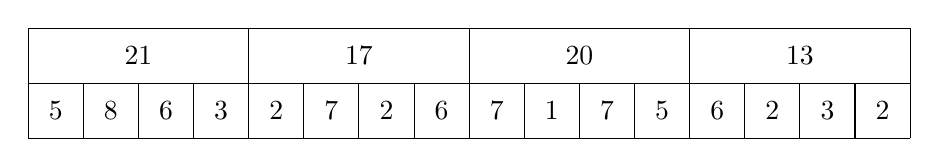
\begin{tikzpicture}[scale=0.7]
\draw (0,0) grid (16,1);

\draw (0,1) rectangle (4,2);
\draw (4,1) rectangle (8,2);
\draw (8,1) rectangle (12,2);
\draw (12,1) rectangle (16,2);

\node at (0.5, 0.5) {5};
\node at (1.5, 0.5) {8};
\node at (2.5, 0.5) {6};
\node at (3.5, 0.5) {3};
\node at (4.5, 0.5) {2};
\node at (5.5, 0.5) {7};
\node at (6.5, 0.5) {2};
\node at (7.5, 0.5) {6};
\node at (8.5, 0.5) {7};
\node at (9.5, 0.5) {1};
\node at (10.5, 0.5) {7};
\node at (11.5, 0.5) {5};
\node at (12.5, 0.5) {6};
\node at (13.5, 0.5) {2};
\node at (14.5, 0.5) {3};
\node at (15.5, 0.5) {2};

\node at (2, 1.5) {21};
\node at (6, 1.5) {17};
\node at (10, 1.5) {20};
\node at (14, 1.5) {13};

\end{tikzpicture}
\end{center}

When a value in the array changes,
we have to calculate the sum of the corresponding
block again:

\begin{center}
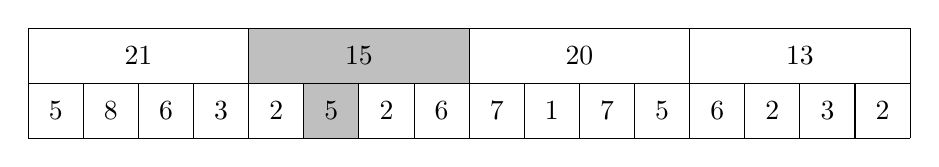
\begin{tikzpicture}[scale=0.7]
\fill[color=lightgray] (5,0) rectangle (6,1);
\draw (0,0) grid (16,1);

\fill[color=lightgray] (4,1) rectangle (8,2);
\draw (0,1) rectangle (4,2);
\draw (4,1) rectangle (8,2);
\draw (8,1) rectangle (12,2);
\draw (12,1) rectangle (16,2);

\node at (0.5, 0.5) {5};
\node at (1.5, 0.5) {8};
\node at (2.5, 0.5) {6};
\node at (3.5, 0.5) {3};
\node at (4.5, 0.5) {2};
\node at (5.5, 0.5) {5};
\node at (6.5, 0.5) {2};
\node at (7.5, 0.5) {6};
\node at (8.5, 0.5) {7};
\node at (9.5, 0.5) {1};
\node at (10.5, 0.5) {7};
\node at (11.5, 0.5) {5};
\node at (12.5, 0.5) {6};
\node at (13.5, 0.5) {2};
\node at (14.5, 0.5) {3};
\node at (15.5, 0.5) {2};

\node at (2, 1.5) {21};
\node at (6, 1.5) {15};
\node at (10, 1.5) {20};
\node at (14, 1.5) {13};

\end{tikzpicture}
\end{center}

Any sum in the array can be calculated as a combination
of single values in the array and the sums of the
blocks between them:

\begin{center}
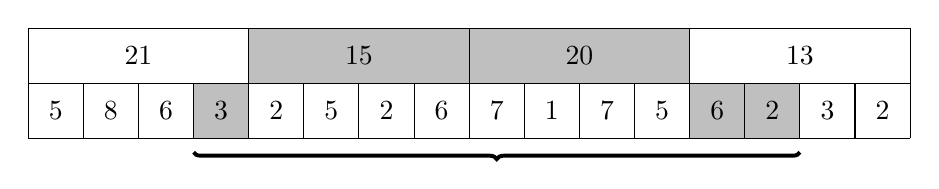
\begin{tikzpicture}[scale=0.7]
\fill[color=lightgray] (3,0) rectangle (4,1);
\fill[color=lightgray] (12,0) rectangle (13,1);
\fill[color=lightgray] (13,0) rectangle (14,1);
\draw (0,0) grid (16,1);

\fill[color=lightgray] (4,1) rectangle (8,2);
\fill[color=lightgray] (8,1) rectangle (12,2);
\draw (0,1) rectangle (4,2);
\draw (4,1) rectangle (8,2);
\draw (8,1) rectangle (12,2);
\draw (12,1) rectangle (16,2);

\node at (0.5, 0.5) {5};
\node at (1.5, 0.5) {8};
\node at (2.5, 0.5) {6};
\node at (3.5, 0.5) {3};
\node at (4.5, 0.5) {2};
\node at (5.5, 0.5) {5};
\node at (6.5, 0.5) {2};
\node at (7.5, 0.5) {6};
\node at (8.5, 0.5) {7};
\node at (9.5, 0.5) {1};
\node at (10.5, 0.5) {7};
\node at (11.5, 0.5) {5};
\node at (12.5, 0.5) {6};
\node at (13.5, 0.5) {2};
\node at (14.5, 0.5) {3};
\node at (15.5, 0.5) {2};

\node at (2, 1.5) {21};
\node at (6, 1.5) {15};
\node at (10, 1.5) {20};
\node at (14, 1.5) {13};

\draw [decoration={brace}, decorate, line width=0.5mm] (14,-0.25) -- (3,-0.25);

\end{tikzpicture}
\end{center}

We can change a value in $O(1)$ time,
because we only have to change the sum of a single block.
A sum in a range consists of three parts:

\begin{itemize}
\item first, there are $O(\sqrt n)$ single values
\item then, there are $O(\sqrt n)$ consecutive blocks
\item finally, there are $O(\sqrt n)$ single values
\end{itemize}

Calculating each sum takes $O(\sqrt n)$ time,
so the total complexity for calculating the sum
of values in any range is $O(\sqrt n)$.

The reason why we use the parameter $\sqrt n$ is that
it balances two things:
for example, an array of $n$ elements is divided
into $\sqrt n$ blocks, each of which contains
$\sqrt n$ elements.
In practice, it is not needed to use exactly
the parameter $\sqrt n$ in algorithms, but it may be better to
use parameters $k$ and $n/k$ where $k$ is
larger or smaller than $\sqrt n$.

The best parameter depends on the problem
and input.
For example, if an algorithm often goes through
blocks but rarely iterates elements inside
blocks, it may be good to divide the array into
$k < \sqrt n$ blocks, each of which contains $n/k > \sqrt n$
elements.

\section{Batch processing}

\index{batch processing}

In \key{batch processing}, the operations of an
algorithm are divided into batches,
and each batch will be processed separately.
Between the batches some precalculation is done
to process the future operations more efficiently.

In a square root algorithm, $n$ operations are
divided into batches of size $O(\sqrt n)$,
and the number of both batches and operations in each
batch is $O(\sqrt n)$.
This balances the precalculation time between
the batches and the time needed for processing
the batches.

As an example, let's consider a problem
where a grid of size $k \times k$
initially consists of white squares.
Our task is to perform $n$ operations,
each of which is one of the following:
\begin{itemize}
\item
paint square $(y,x)$ black
\item
find the nearest black square to
square $(y,x)$ where the distance
between squares $(y_1,x_1)$ and $(y_2,x_2)$
is $|y_1-y_2|+|x_1-x_2|$
\end{itemize}

The solution is to divide the operations into
$O(\sqrt n)$ batches, each of which consists
of $O(\sqrt n)$ operations.
At the beginning of each batch,
we calculate for each square in the grid
the smallest distance to a black square.
This can be done in $O(k^2)$ time using breadth-first search.

When processing a batch, we maintain a list of squares
that have been painted black in the current batch.
Now, the distance from a square to the nearest black
square is either the precalculated distance or the distance
to a square that has been painted black in the current batch.

The algorithm works in
$O((k^2+n) \sqrt n)$ time.
First, between the batches,
there are $O(\sqrt n)$ searches that each take
$O(k^2)$ time.
Second, the total number of processed
squares is $O(n)$, and at each square,
we go through a list of $O(\sqrt n)$ squares
in a batch.

If the algorithm would perform a breadth-first search
at each operation, the complexity would be
$O(k^2 n)$.
And if the algorithm would go through all painted
squares at each operation,
the complexity would be $O(n^2)$.
The square root algorithm combines these complexities,
and turns the factor $n$ into $\sqrt n$.

\section{Case processing}

\index{case processing}

In \key{case processing}, an algorithm has
specialized subalgorithms for different cases that
may appear during the algorithm.
Typically, one part is efficient for
small parameters, and another part is efficient
for large parameters, and the turning point is
about $\sqrt n$.

As an example, let's consider a problem where
we are given a tree that contains $n$ nodes,
each with some color. Our task is to find two nodes
that have the same color and the distance
between them is as large as possible.

The problem can be solved by going through all
colors one after another, and for each color,
finding two nodes of that color whose distance is
maximum.
For a fixed color, a subalgorithm will be used
that depends on the number of nodes of that color.
Let's assume that the current color is $x$
and there are $c$ nodes whose color is $x$.
There are two cases:

\subsubsection*{Case 1: $c \le \sqrt n$}

If the number of nodes is small,
we go through all pairs of nodes whose
color is $x$ and select the pair that
has the maximum distance.
For each node, we have calculate the distance
to $O(\sqrt n)$ other nodes (see 18.3),
so the total time needed for processing all
nodes in case 1 is $O(n \sqrt n)$.

\subsubsection*{Case 2: $c > \sqrt n$}

If the number of nodes is large,
we traverse through the whole tree
and calculate the maximum distance between
two nodes with color $x$.
The time complexity of the tree traversal is $O(n)$,
and this will be done at most $O(\sqrt n)$ times,
so the total time needed for case 2 is
$O(n \sqrt n)$.\\\\
\noindent
The time complexity of the algorithm is $O(n \sqrt n)$,
because both case 1 and case 2 take $O(n \sqrt n)$ time.

\section{Mo's algorithm}

\index{Mo's algorithm}

\key{Mo's algorithm} can be used in many problems
that require processing range queries in 
a \emph{static} array.
Before processing the queries, the algorithm
sorts them in a special order which guarantees
that the algorithm runs efficiently.

At each moment in the algorithm, there is an active
subarray and the algorithm maintains the answer
for a query to that subarray.
The algorithm processes the given queries one by one,
and always changes the active subarray
by inserting and removing elements
so that it corresponds to the current query.
The time complexity of the algorithm is
$O(n \sqrt n f(n))$ when there are $n$ queries
and each insertion and removal of an element
takes $O(f(n))$ time.

The essential trick in Mo's algorithm is that
the queries are processed in a special order,
which makes the algorithm efficient.
The array is divided into blocks of $k=O(\sqrt n)$
elements, and the queries are sorted primarily by
the index of the block that contains the first element
of the query, and secondarily by the index of the
last element of the query.
It turns out that using this order, the algorithm
only performs $O(n \sqrt n)$ operations,
because the left border of the subarray moves
$n$ times $O(\sqrt n)$ steps,
and the right border of the subarray moves
$\sqrt n$ times $O(n)$ steps. Thus, both the
borders move a total of $O(n \sqrt n)$ steps.

\subsubsection*{Example}

As an example, let's consider a problem
where we are given a set of subarrays in an array,
and our task is to calculate for each subarray
the number of distinct elements in the subarray.

In Mo's algorithm, the queries are always sorted
in the same way, but the way the answer for the query
is maintained depends on the problem.
In this problem, we can maintain an array 
\texttt{c} where $\texttt{c}[x]$
indicates how many times an element $x$
occurs in the active subarray.

When we move from a query to another query,
the active subarray changes.
For example, if the current subarray is
\begin{center}
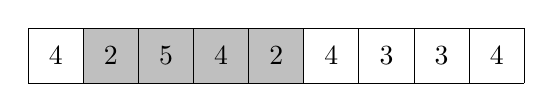
\begin{tikzpicture}[scale=0.7]
\fill[color=lightgray] (1,0) rectangle (5,1);
\draw (0,0) grid (9,1);
\node at (0.5, 0.5) {4};
\node at (1.5, 0.5) {2};
\node at (2.5, 0.5) {5};
\node at (3.5, 0.5) {4};
\node at (4.5, 0.5) {2};
\node at (5.5, 0.5) {4};
\node at (6.5, 0.5) {3};
\node at (7.5, 0.5) {3};
\node at (8.5, 0.5) {4};
\end{tikzpicture}
\end{center}
and the next subarray is
\begin{center}
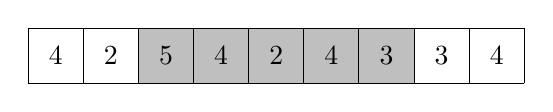
\begin{tikzpicture}[scale=0.7]
\fill[color=lightgray] (2,0) rectangle (7,1);
\draw (0,0) grid (9,1);
\node at (0.5, 0.5) {4};
\node at (1.5, 0.5) {2};
\node at (2.5, 0.5) {5};
\node at (3.5, 0.5) {4};
\node at (4.5, 0.5) {2};
\node at (5.5, 0.5) {4};
\node at (6.5, 0.5) {3};
\node at (7.5, 0.5) {3};
\node at (8.5, 0.5) {4};
\end{tikzpicture}
\end{center}
there will be three steps:
the left border moves one step to the left,
and the right border moves two steps to the right.

After each step, we update the
array \texttt{c}.
If an element $x$ is added to the subarray,
the value
$\texttt{c}[x]$ increases by one,
and if an element $x$ is removed from the subarray,
the value $\texttt{c}[x]$ decreases by one.
If after an insertion
$\texttt{c}[x]=1$,
the answer for the query increases by one,
and if after a removal $\texttt{c}[x]=0$,
the answer for the query decreases by one.

In this problem, the time needed to perform
each step is $O(1)$, so the total time complexity
of the algorithm is $O(n \sqrt n)$.